% Minimal example sheet showing the template style.
% Compile from this folder, e.g.:  latexmk -pdf example.tex   (or pdflatex example.tex)
%
% The bot does NOT use this file — at /build it generates its own ex<NN>/ex<NN>.tex from
% the images picked in Discord. This is just a human-readable reference for the layout and
% a smoke test that exercise.sty compiles on a fresh TeX install.
\documentclass[a4paper,11pt]{scrartcl}

% Define \exerciseTitle before loading the package (exercise.sty renews it), matching what
% the bot emits — so this example compiles cleanly out of the box.
\providecommand{\exerciseTitle}{}
\usepackage{exercise}
\setExerciseSheet{01} % <-- sheet number (zero-padded), e.g. 01
\exerciseMakeHeaders

\begin{document}
\section*{Exercise 1}

% A whole-exercise figure (no sub-part label), like a single uploaded photo.
\begin{figure}[!htb]
    \centering
    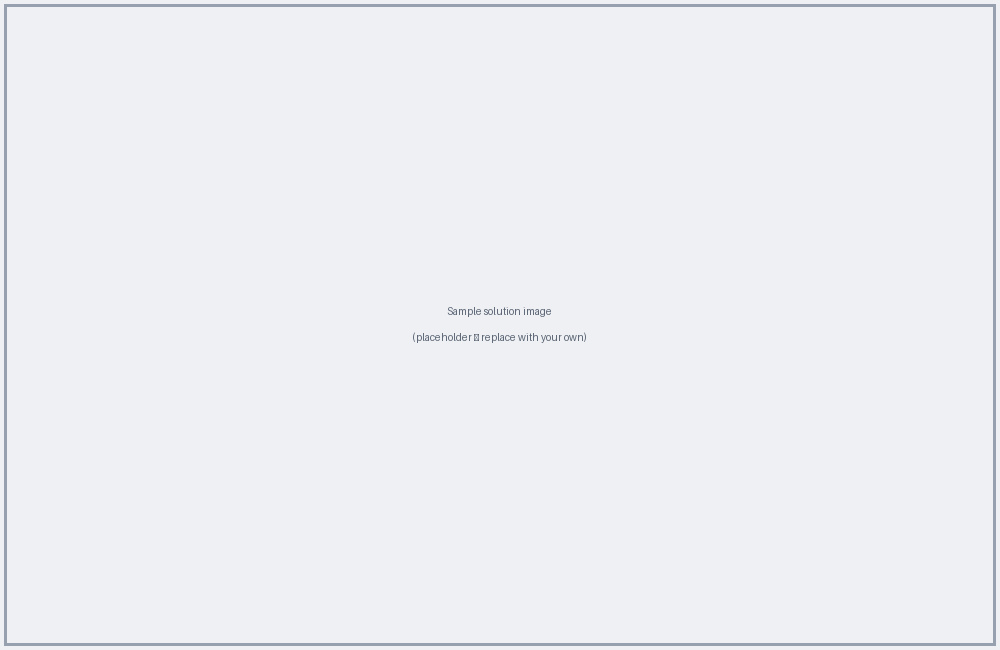
\includegraphics[width=0.95\linewidth]{sample.png}
\end{figure}

\newpage
\section*{Exercise 2}

% A sub-part label above a figure, like the bot emits for "a: <image>".
\paragraph{(a)}
\begin{figure}[!htb]
    \centering
    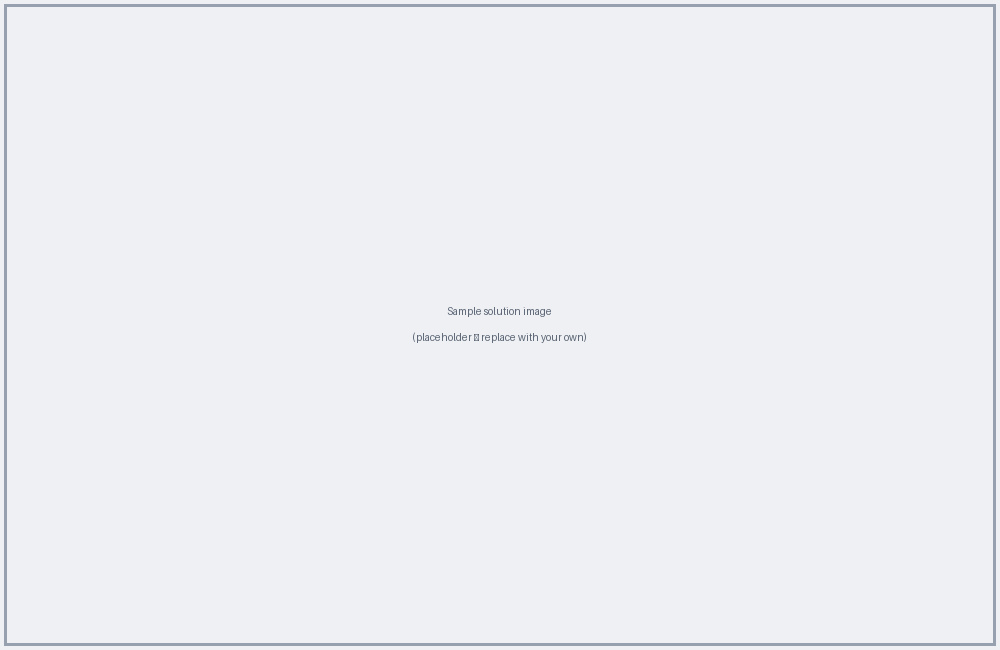
\includegraphics[width=0.95\linewidth]{sample.png}
\end{figure}

\paragraph{(b)}
\begin{figure}[!htb]
    \centering
    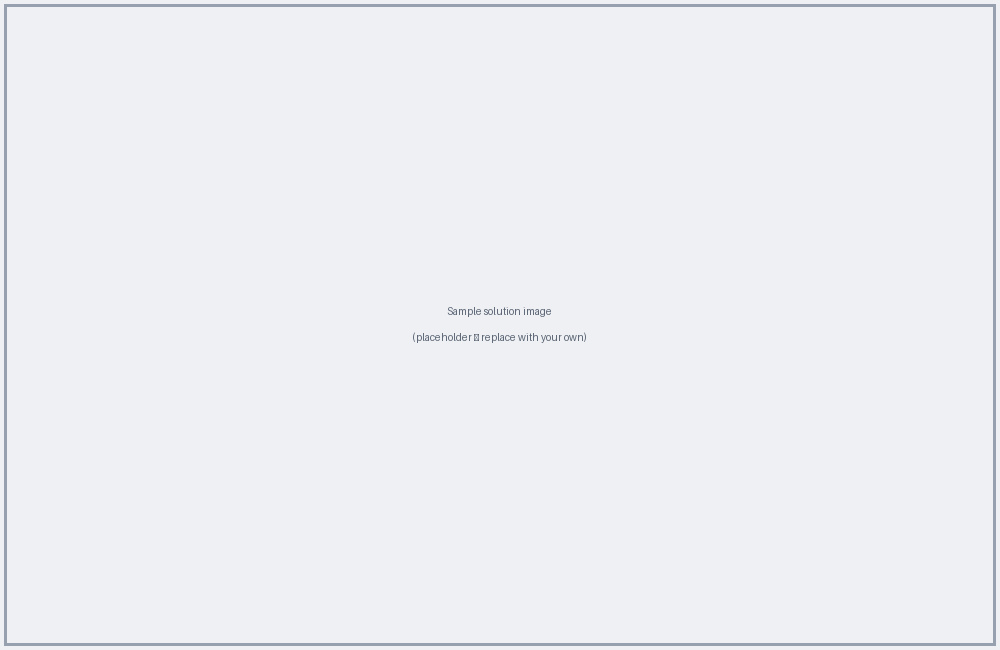
\includegraphics[width=0.95\linewidth]{sample.png}
\end{figure}

\end{document}
